\documentclass{article}
\usepackage{circuitikz}
\usetikzlibrary{arrows.meta, positioning, calc, shapes.geometric}

\tikzset{
  springpot/.pic={
    \node[draw, diamond, minimum width=8mm, minimum height=10mm, inner sep=1pt, line width=2pt] (d) {};
    \path (d.center) coordinate (-center);
    \path (d.west)   coordinate (-west);
    \path (d.east)   coordinate (-east);
  }
}

\begin{document}

% transfer function schematic
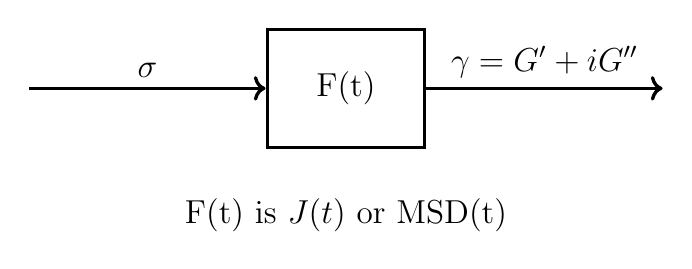
\begin{tikzpicture}[
    node distance=2cm,
    every node/.style={font=\large},
    block/.style={draw, rectangle, minimum width=2cm, minimum height=1.5cm, very thick},
    input/.style={-Stealth, thick},
    output/.style={-Stealth, thick}
    ]
    \node[block] (f) {F(t)};
    \node[below=0.5cm of f] (note) {F(t) is $J(t)$ or MSD(t)};
    \draw[<-,very thick] ($(f.west) + (0,0)$) -- ++(-3,0) node[midway, above] {$\sigma$};
    \draw[->,very thick] ($(f.east) + (0,0)$) -- ++(3,0) node[midway, above] {$\gamma = G' + iG''$};
\end{tikzpicture}

% Maxwell model
\begin{circuitikz}[european, thick, >=latex]
  \draw (0,0) to[spring, l=$G$] (2,0);
  \draw (2,0) to[damper, l=$\eta$] (4,0);
  \draw (0,0) -- ++(-0.7,0);
  \draw (4,0) -- ++(0.7,0);
\end{circuitikz}

% Kelvin-Voigt model
\begin{circuitikz}[european, thick, >=latex]
    \coordinate (L) at (0,-0.6);
    \coordinate (R) at (4,-0.6);
    \draw (L) -- ++(-0.7,0);
    \draw (R) -- ++(0.7,0);
    \draw (L) |- (0,0) to[spring, l=$G$] (4,0) -| (R);
    \draw (L) |- (0,-1.2) to[damper, l=$\eta$] (4,-1.2) -| (R);
\end{circuitikz}

% Fractional Maxwell model
\begin{circuitikz}[european, thick, >=latex]
  \path (0,0) coordinate (start);
  \path (start) ++(1.7,0) pic (sp1) {springpot};
  \node[above=0.5 of sp1-center] {$\mathbb{V},\alpha$};
  \path (sp1-east) ++(1.7,0) pic (sp2) {springpot};
  \node[above=0.5 of sp2-center] {$\mathbb{G},\beta$};
  \draw (start) -- (sp1-west)
        (sp1-east) -- (sp2-west)
        (sp2-east) -- (5.5,0);
\end{circuitikz}

% Johnson-Segalman model
\begin{circuitikz}[european, thick, >=latex]
    \coordinate (L) at (0,-0.6);
    \coordinate (R) at (6,-0.6);
    \draw (L) -- ++(-0.7,0);
    \draw (R) -- ++(0.7,0);
    \draw (L) |- (0,0) to[damper, l=$\eta_s$] (6,0) -| (R);
    \draw (L) |- (0,-1.2) coordinate (B1)
          to[spring, l=$G$] (3,-1.2) coordinate (B2)
          to[damper, l=$\eta$] (6,-1.2) -| (R);
\end{circuitikz}

\end{document}
